\documentclass[a4paper,12pt]{article}

% --- Pakiety ---
\usepackage[polish]{babel}
\usepackage[utf8]{inputenc}
\usepackage[T1]{fontenc}
\usepackage{geometry}
\usepackage{graphicx}
\usepackage{float}     
\usepackage{booktabs}  
\usepackage{amsmath}
\usepackage{hyperref}  
\usepackage{caption}

% --- DODANO PAKIET DO CENTROWANIA TABEL ---
\usepackage{etoolbox} 
% Ta komenda mówi: "Na początku każdego środowiska 'table' wstaw \centering"
\AtBeginEnvironment{table}{\centering}
% ------------------------------------------

% --- Ustawienia marginesów ---
\geometry{
 a4paper,
 total={170mm,257mm},
 left=20mm,
 top=20mm,
}

% --- Dane dokumentu ---
\title{\textbf{Sprawozdanie z Laboratorium 5}}
\author{Wiktor Zoga}
\date{\today}

\begin{document}

\maketitle
\newpage

% =================================================================
% ZADANIE 1
% =================================================================
\section{Zadanie 1: Regresja Liniowa na Danych Medycznych}

Celem zadania była analiza zależności poziomu satysfakcji pacjenta od jego wieku, ciężkości choroby oraz poziomu niepokoju. Wykorzystano model regresji liniowej wielokrotnej.

\subsection{Estymacja parametrów i testy istotności (a, c)}
Poniższa tabela przedstawia oszacowane współczynniki regresji, ich błędy standardowe oraz wyniki testów t-Studenta.

% Teraz ta tabela wycentruje się sama dzięki komendzie w preambule!
\begin{table}[H]
\caption{Estymatory, testy istotności i przedziały ufności (Zadanie 1a, 1c)}
\label{tab:zad1_coeffs}
\begin{tabular}{lccccccc}
\toprule
Zmienna & Współczynnik & Błąd Std & Statystyka t & p-value & 95\% CI Dolny & 95\% CI Górny \\
\midrule
const & 1.0532 & 0.6138 & 1.7160 & 0.0935 & -0.1854 & 2.2919 \\
Age & -0.0059 & 0.0031 & -1.8973 & 0.0647 & -0.0121 & 3.73e-04 \\
Severity & 0.0019 & 0.0058 & 0.3332 & 0.7407 & -0.0097 & 0.0136 \\
Anxiety & 0.0301 & 0.0093 & 3.2569 & 0.0022 & 0.0115 & 0.0488 \\
\bottomrule
\end{tabular}
\end{table}


\textbf{Wnioski:} 
Na podstawie p-wartości można stwierdzić, które zmienne są istotne statystycznie przy poziomie istotności $\alpha=0.05$. Przedziały ufności wskazują zakres, w którym z 95\% prawdopodobieństwem znajduje się prawdziwa wartość parametru.

\subsection{Dopasowanie modelu (b)}
Ocenę jakości dopasowania modelu oraz wynik ogólnego testu F przedstawiono poniżej.

\begin{table}[H]
\caption{Ocena dopasowania modelu i ogólny test F (Zadanie 1b)}
\label{tab:zad1_fit}
\begin{tabular}{lcccccc}
\toprule
R-kwadrat & Adj. R-kwadrat & Statystyka F & p-value (F) & df Model & df Reszty \\
\midrule
0.5415 & 0.5088 & 16.5376 & 3.04e-07 & 3.0000 & 42.0000 \\
\bottomrule
\end{tabular}
\end{table}


Wysoka wartość statystyki F (oraz p-value < 0.05) świadczy o tym, że model jako całość jest istotny statystycznie.

\subsection{Diagnostyka reszt (d)}
W celu weryfikacji założeń modelu przeanalizowano rozkład reszt.

\begin{figure}[H]
    \centering
    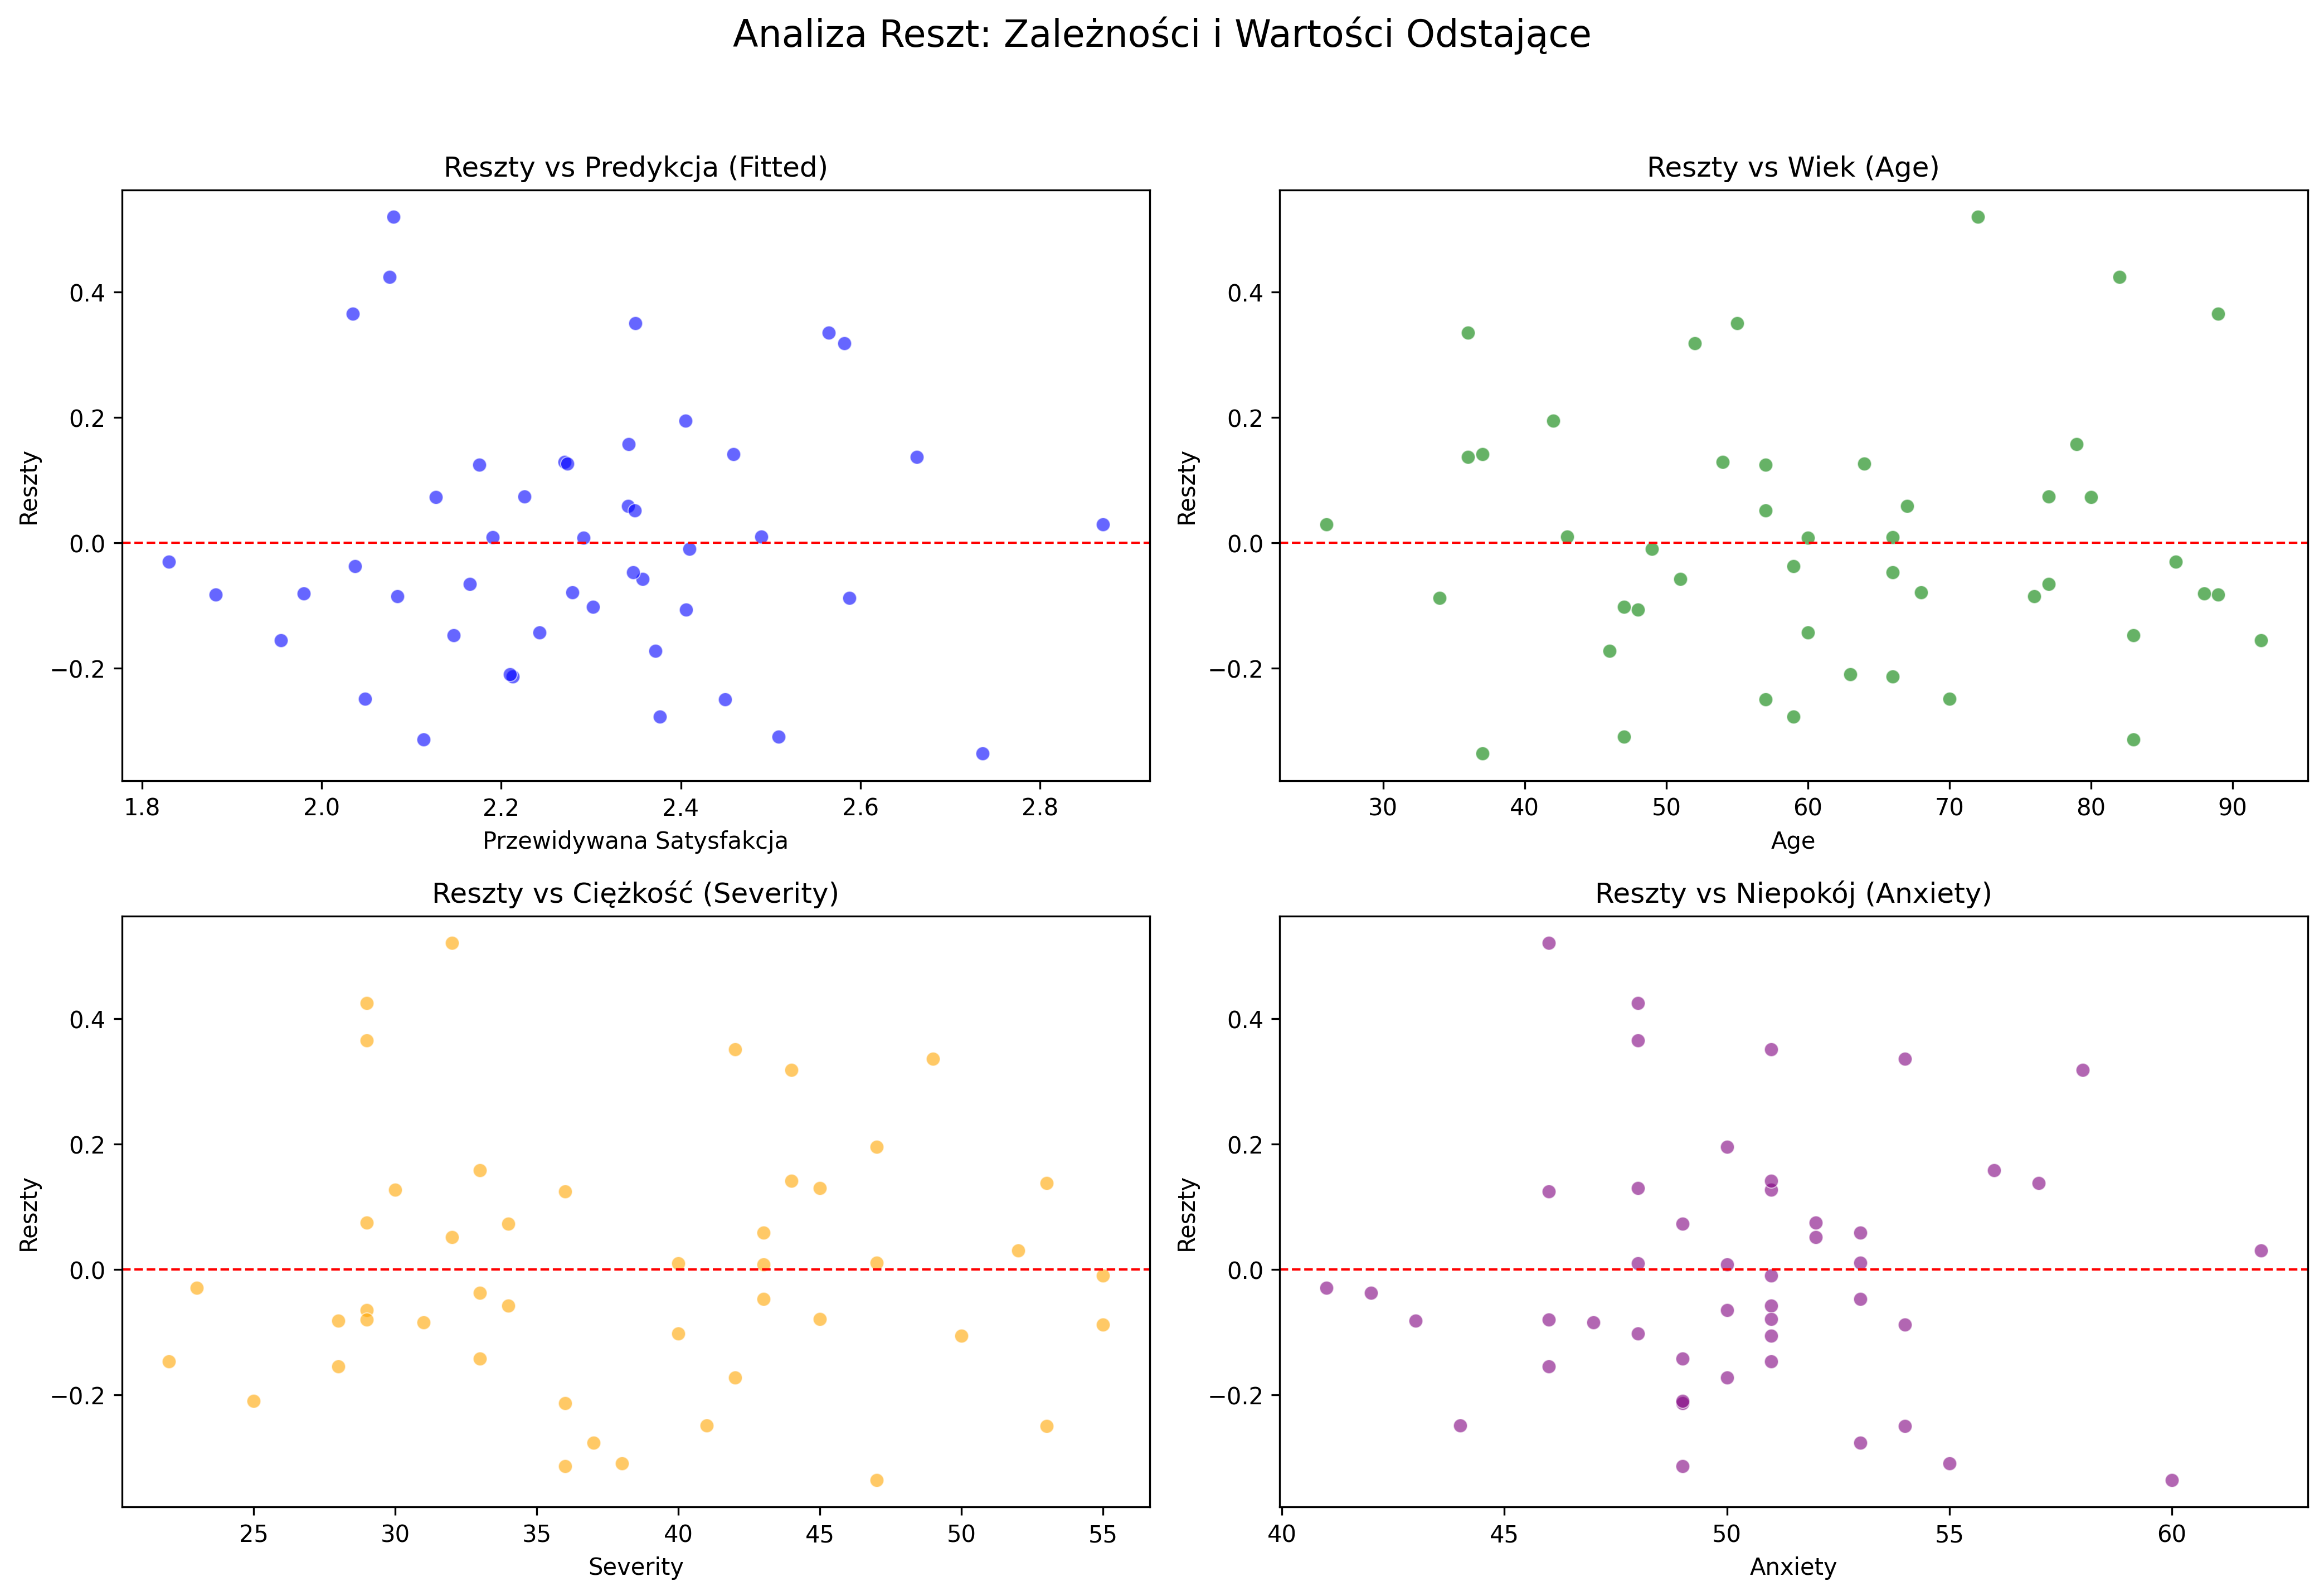
\includegraphics[width=1.0\textwidth]{../zad1/wykres_zad1_reszty.png}
    \caption{Wykresy rozrzutu reszt względem wartości dopasowanych oraz zmiennych objaśniających.}
    \label{fig:reszty_scatter}
\end{figure}

Wykresy nie wykazują wyraźnych struktur, co sugeruje liniowość zależności. Aby sprawdzić normalność rozkładu reszt, sporządzono histogram oraz wykres kwantylowy (Q-Q plot).

\begin{figure}[H]
    \centering
    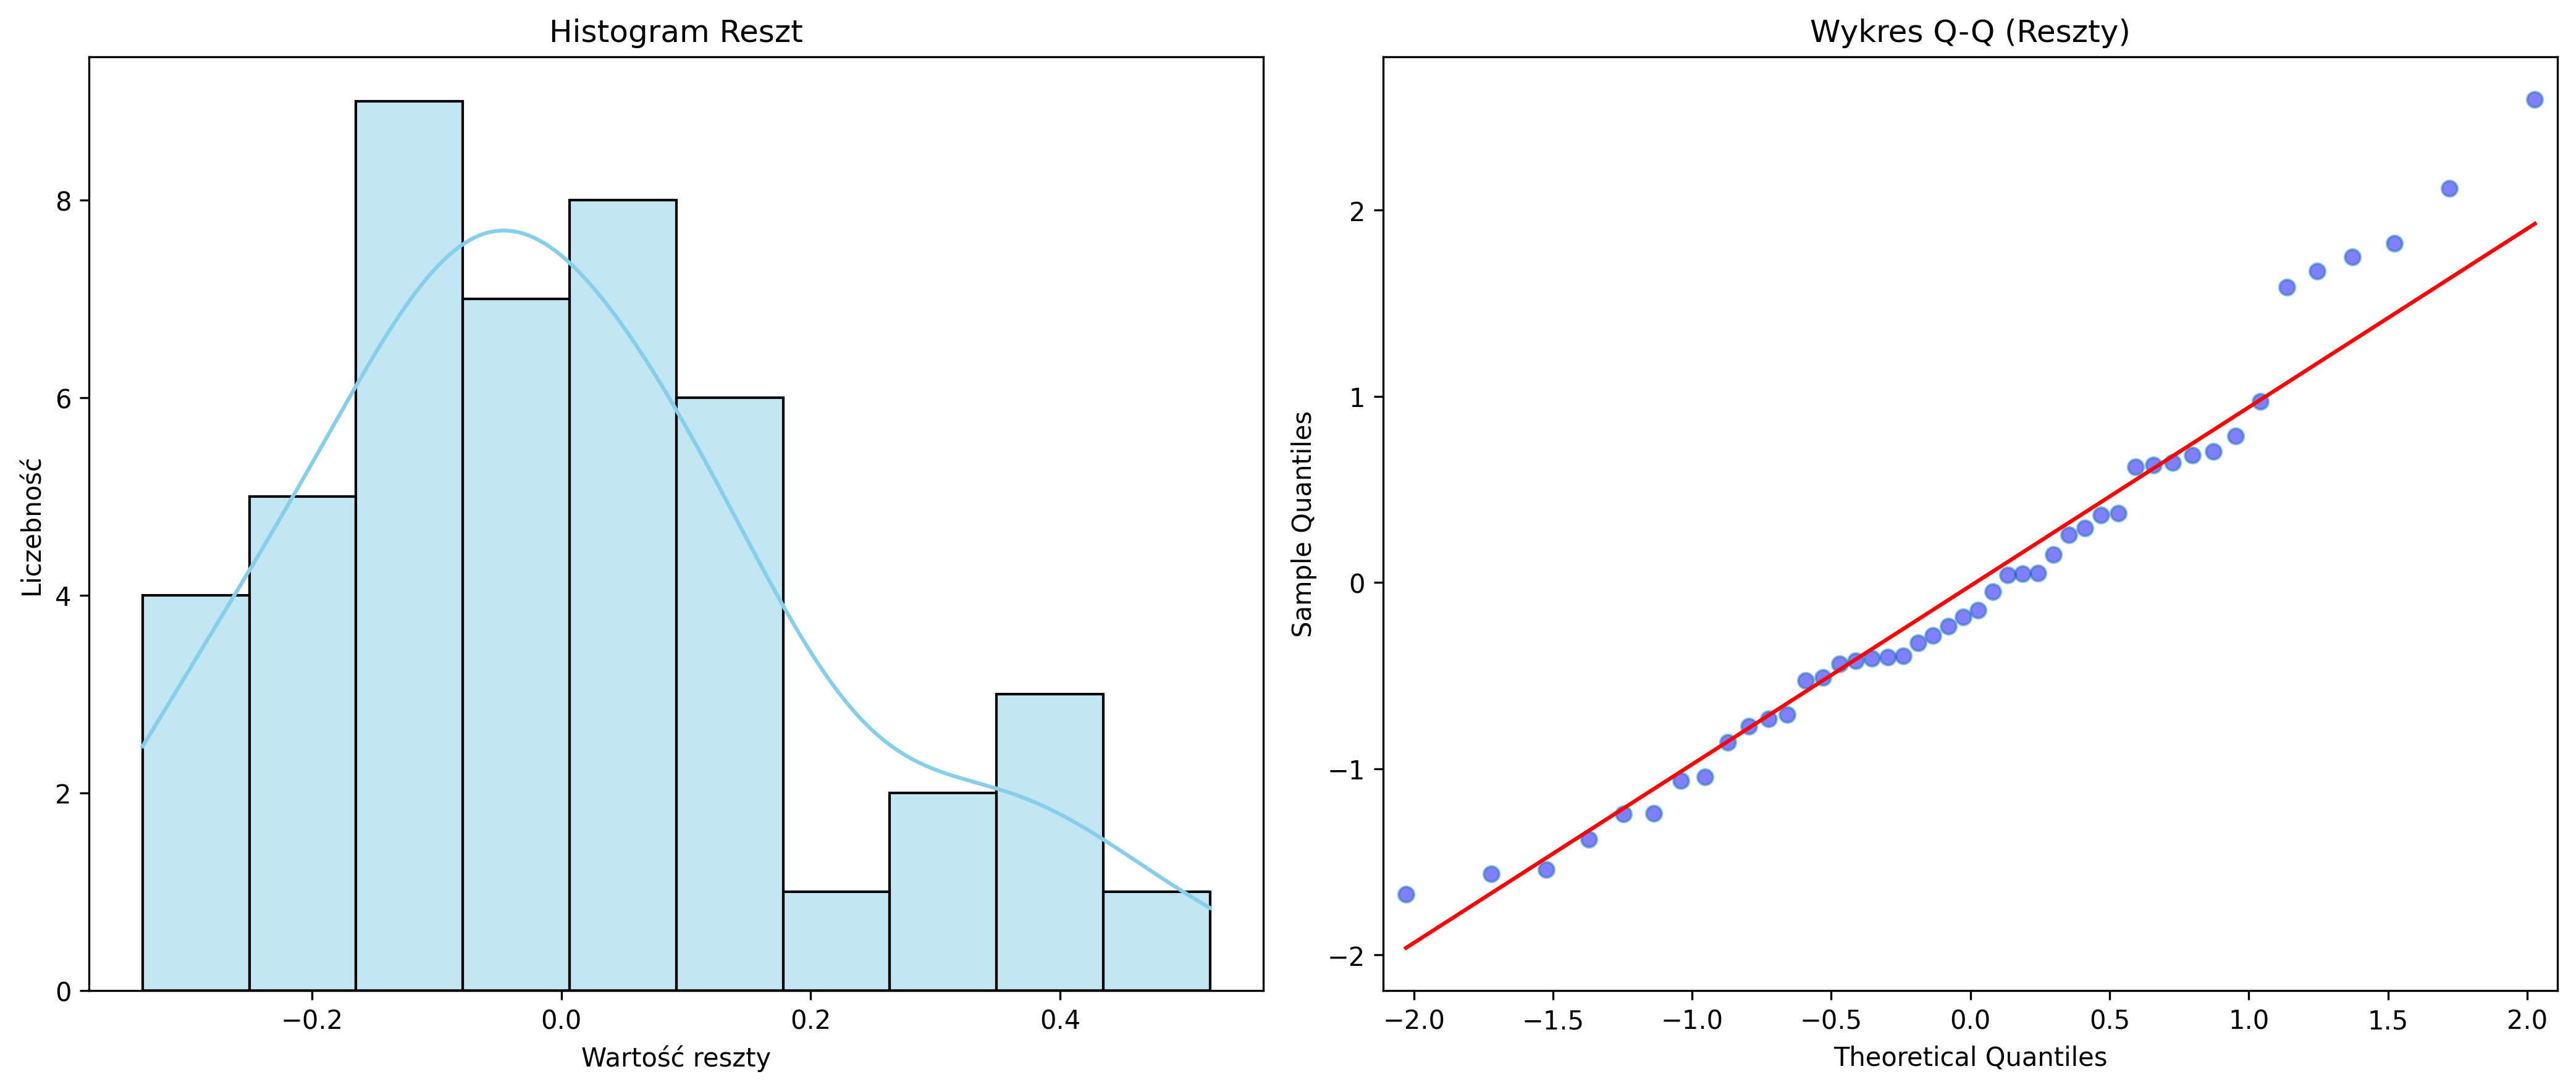
\includegraphics[width=0.9\textwidth]{../zad1/wykres_zad1_normalnosc.png}
    \caption{Diagnostyka normalności reszt.}
    \label{fig:reszty_norm}
\end{figure}

Wynik testu statystycznego Shapiro-Wilka:

\begin{table}[H]
\caption{Test normalności reszt Shapiro-Wilka (Zadanie 1d)}
\label{tab:zad1_shapiro}
\begin{tabular}{lcccc}
\toprule
Test & Statystyka W & p-value & Decyzja (alpha=0.05) \\
\midrule
Shapiro-Wilk & 0.9629 & 0.1481 & Normality \\
\bottomrule
\end{tabular}
\end{table}


\subsection{Porównanie modeli (e)}
Przeprowadzono test F w celu sprawdzenia, czy dodanie zmiennych \textit{Severity} i \textit{Anxiety} do modelu zawierającego tylko \textit{Age} istotnie poprawia dopasowanie.

% =================================================================
% ZADANIE 2
% =================================================================
\newpage
\section{Zadanie 2: Wpływ wysokiego wymiaru danych}

W zadaniu sprawdzamy, jak zachowuje się regresja, gdy mamy bardzo dużo zmiennych ($p=950$) w stosunku do liczby obserwacji ($n=1000$). Tylko pierwsze 5 zmiennych faktycznie wpływa na wynik ($\beta=3$), reszta to szum.

\subsection{Punkt B: Modele oparte na pierwszych k kolumnach}
W tym kroku dodawaliśmy kolejne zmienne zgodnie z ich kolejnością w pliku.

\begin{table}[H]
\caption{Wyniki regresji dla punktu b}
\label{tab:zad2_b}
\begin{tabular}{lccccccc}
\toprule
k & SSE & MSE & AIC & p X1 & p X2 & FP \\
\midrule
1 & 1361.0054 & 0.3360 & 310.2237 & 0.0000 & --- & 0 \\
2 & 1282.2922 & 0.8223 & 252.6492 & 0.0000 & 0.0000 & 0 \\
5 & 975.3407 & 7.3033 & -14.9684 & 0.0000 & 0.0000 & 0 \\
10 & 971.9580 & 10.6861 & -8.4427 & 0.0000 & 0.0000 & 0 \\
50 & 937.8749 & 44.7691 & 35.8613 & 0.0000 & 0.0000 & 0 \\
100 & 873.2252 & 109.4189 & 64.4382 & 0.0000 & 0.0000 & 6 \\
500 & 489.2595 & 493.3845 & 285.1378 & 1.57e-09 & 2.94e-11 & 28 \\
950 & 43.8282 & 938.8158 & -1227.4775 & 0.2951 & 0.1696 & 18 \\
\bottomrule
\end{tabular}
\end{table}


\textbf{Obserwacje:}
\begin{itemize}
    \item SSE (błąd dopasowania) zawsze spada, gdy dodajemy zmienne. Jest to jednak złudne – przy $k=950$ błąd prawie znika ($43.82$), ale model przestaje widzieć istotność prawdziwych zmiennych ($X_1, X_2$).
    \item AIC poprawnie wskazuje najlepszy model dla $k=5$ (wartość $-14.96$). Jednak przy $k=950$ AIC "wariuje" i pokazuje ogromną wartość ujemną, co błędnie sugeruje idealny model.
\end{itemize}

\subsection{Punkt C: Wybór zmiennych z największymi współczynnikami}
Tutaj wybieraliśmy zmienne nie po kolei, ale te, które miały najwyższe wyliczone współczynniki $\hat{\beta}$ w pełnym modelu.

\begin{table}[H]
\caption{Wyniki regresji dla punktu c}
\label{tab:zad2_c}
\begin{tabular}{lcccccc}
\toprule
k & SSE & MSE & AIC & TP & FP \\
\midrule
1 & 1395.1811 & 370.4290 & 335.0242 & 1 & 0 \\
2 & 1240.2176 & 281.2722 & 219.2868 & 2 & 0 \\
5 & 1238.8119 & 283.7671 & 224.1528 & 2 & 0 \\
10 & 1212.9137 & 298.9966 & 213.0254 & 2 & 1 \\
50 & 1075.3234 & 232.2150 & 172.6214 & 3 & 5 \\
100 & 932.9998 & 209.8877 & 130.6497 & 4 & 13 \\
500 & 263.8108 & 718.8333 & -332.5232 & 5 & 332 \\
950 & 43.8282 & 938.8158 & -1227.4775 & 2 & 18 \\
\bottomrule
\end{tabular}
\end{table}


\textbf{Obserwacje:}
Wybieranie zmiennych na podstawie tego, jak wysokie mają współczynniki, to "oszukiwanie" statystyki. Widzimy to po bardzo dużej liczbie fałszywych odkryć (FP) – np. dla $k=500$ model uznał aż 332 nieistotnych zmiennych za ważne.

\subsection{Punkt D: Wyniki z 1000 symulacji}
Tabela poniżej pokazuje średnie wyniki z powtórzenia całego eksperymentu 1000 razy.

\begin{table}[H]
\caption{Wyniki symulacji (punkt d)}
\label{tab:zad2_d}
\begin{tabular}{lccccccc}
\toprule
k & Pow X1 (B) & Pow X2 (B) & E(FD) (B) & Pow X1 (C) & Pow X2 (C) & E(FD) (C) \\
\midrule
1 & 1.0000 & 0.0000 & 0.0000 & 0.1070 & 0.0900 & 0.0690 \\
2 & 1.0000 & 1.0000 & 0.0000 & 0.1570 & 0.1600 & 0.1300 \\
5 & 1.0000 & 1.0000 & 0.0000 & 0.2800 & 0.2600 & 0.3790 \\
10 & 1.0000 & 1.0000 & 0.2350 & 0.3590 & 0.3410 & 0.8240 \\
50 & 1.0000 & 1.0000 & 2.2120 & 0.5690 & 0.5760 & 4.8160 \\
100 & 1.0000 & 1.0000 & 4.7000 & 0.6760 & 0.6800 & 11.4960 \\
500 & 1.0000 & 1.0000 & 24.8030 & 0.9100 & 0.9190 & 286.5000 \\
950 & 0.4510 & 0.5180 & 48.9320 & 0.4510 & 0.5180 & 48.9320 \\
\bottomrule
\end{tabular}
\end{table}


\paragraph{Wyniki i wnioski:}
\begin{itemize}
    \item \textbf{Słaba wykrywalność w punkcie C:} Jeśli wybieramy zmienne "najsilniejsze" z danych, często pomijamy te prawdziwe. Moc dla $k=1$ spadła z 100\% (w punkcie B) do zaledwie 10\% (w punkcie C).
    \item \textbf{Zalew fałszywych odkryć:} Punkt C generuje ogromną liczbę błędów (E[FD]). Szukając na siłę najlepszych zmiennych, po prostu wybieramy te, które przypadkiem zgrały się z szumem.
    \item \textbf{Problem $k=950$:} Gdy zmiennych jest prawie tyle co danych, testy przestają działać. Nawet w "uczciwym" punkcie B moc wykrywania $X_1$ spada do ok. 45\%.
\end{itemize}

\subsection{Wnioski końcowe}
\begin{itemize}
    \item \textbf{Dlaczego tak się dzieje?} W zadaniu sygnał jest słaby. Wariancja jednej ważnej zmiennej to $3^2 \cdot 0.1^2 = 0.09$, a wariancja błędu to $1.0$. Szum jest więc 11 razy silniejszy niż pojedyncza zmienna.
    \item \textbf{Selekcja zmiennych:} Scenariusz (b) jest bezpieczniejszy, bo nie manipulujemy wyborem. Scenariusz (c) pokazuje, że wybieranie zmiennych "bo mają wysokie wyniki" prowadzi do wyciągania błędnych wniosków z szumu.
    \item \textbf{AIC w wysokim wymiarze:} Przy dużej liczbie zmiennych ($p \approx n$) tradycyjne wskaźniki jak AIC zawodzą – promują zbyt skomplikowane modele, które po prostu "uczą się szumu" na pamięć.
\end{itemize}

\end{document}